\section{The basics of Quantum Monte-Carlo}

\subsection{The basic idea}

\begin{frame}
 Applying the \textit{projection operator} $\OP{P}(\tau)$ on an arbitrary state $\ket{\Psi_T}$ projects the state onto the ground state of $\OP{H}$ as $\tau\to\infty$.  
 \pause
  \begin{align*}
   \onslide<2->{\OP{P}(\tau)\ket{\Psi_T} &= \exp(-(\OP{H} - E_0)\tau)\ket{\Psi_T} \\}
   \onslide<3->{&= \exp(-(\OP{H} - E_0)\tau)\sum_{k} C_k\ket{\Psi_k} \\}
   \onslide<4->{&= \sum_{k} C_k\exp(-(E_k - E_0)\tau) \ket{\Psi_k} \\}
   \onslide<5->{&= C_0\ket{\Psi_0} + \sum_{k=1} C_k\exp(-\Delta E_k\tau) \ket{\Psi_k},}
  \end{align*}

  \onslide<5->where $\Delta E_k > 0$ and $C_k = \braket{\Psi_k}{\Psi_T}$. 

\end{frame}

\begin{frame}
 In other words
 
 \begin{equation}
  \lim_{\tau\to\infty}\bra{\mathbf{r}}\OP{P}(\tau)\ket{\Psi_T} = \braket{\Psi_0}{\Psi_T}\Psi_0(\mathbf{r}).
 \end{equation}

 \pause
 \textbf{Idea}: Use an arbitrary \textit{trial wave function} $\Psi_T(\mathbf{r})$ and perform the projection.
 \shift
 
 \textbf{Problem}: Requires a priori knowledge of the exact ground state energy $E_0$.
 \shift
 
 \textbf{Solution}: Introduce a \textit{trial energy} $E_T(\tau)$. Will work as long as the trial energy drops below $E_1$ at a certain stage (and stays there). 
 
\end{frame}

\begin{frame}
 
 In order to relate the projection process to a \textit{Markov chain} Monte-Carlo process, $\tau$ needs to be split into sequential steps $\delta\tau$. 
 \shift
 
 This is achieved by using the following property of the projection operator
 
 \begin{align*}
  \OP{P}(\tau + \delta\tau) &= \exp(-(\OP{H} - E_T(\tau + \delta\tau))(\tau + \delta\tau)) \\
                            &=  \exp(-(\OP{H} - E_T(\tau + \delta\tau))\delta\tau) \\
                            & \qquad \times\exp(-(\OP{H} - E_T(\tau + \delta\tau))\tau) \\
                            &\simeq \exp(-(\OP{H} - E_T(\tau + \delta\tau))\delta\tau)\OP{P}(\tau),
 \end{align*}

where the relation is approximate due to $E_T$ not being constant.
 
 
 
\end{frame}

\begin{frame}
  Let $\ket{\Phi(\tau)}$ represent $\OP{P}(\tau)\ket{\Psi_T}$. Using the relation from the previous slide reveals
  \pause
  \begin{align*}
   \onslide<2->{\Phi(\mathbf{r}, \tau + \delta\tau) &= \braket{\mathbf{r}}{\Phi(\tau + \delta\tau)} \\ &= \bra{\mathbf{r}}\OP{P}(\tau + \delta\tau)\ket{\Psi_T} \\}
   \onslide<3->{&\simeq  \bra{\mathbf{r}}\exp(-(\OP{H} - E_T)\delta\tau)\OP{P}(\tau)\ket{\Psi_T} \\}
   \onslide<4->{&=\bra{\mathbf{r}}\exp(-(\OP{H} - E_T)\delta\tau)\ket{\Phi(\tau)}  \\}
   \onslide<5->{&= \int_\mathbf{r'}\bra{\mathbf{r}}\exp(-(\OP{H} - E_T)\delta\tau)\ket{\mathbf{r'}}\Phi(\mathbf{r'}, \tau)\mathrm{d}\mathbf{r'},}
  \end{align*}
  
  \pause\pause\pause\pause
  where $\bra{\mathbf{r}}\exp(-(\OP{H} - E_T)\delta\tau)\ket{\mathbf{r'}} \equiv G(\mathbf{r'}, \mathbf{r}; \delta\tau)$ is a \textit{Green's function} interpreted as the transition probability between $\mathbf{r}$ and $\mathbf{r'}$.
    
\end{frame}

\begin{frame}
 \textbf{Idea}: In order to relate the Green's function to well known Markov processes, the exponential is split
 
 \begin{align*}
  \exp(-(\OP{H} - E_T)\delta\tau) &= \exp\left(\frac{1}{2}\nabla^2\delta\tau - (\OP{V} - E_T)\delta\tau\right)\\
     &= \exp\left(\frac{1}{2}\nabla^2\delta\tau\right)\exp( - (\OP{V} - E_T)\delta\tau) \\
     & \qquad  + \mathcal{O}(\delta\tau^2),
 \end{align*}
 
 where the kinetic part describes a diffusion process with diffusion constant $D=\frac{1}{2}$, and the potential part describes a weighting (linear in position space). This is referred to as the \textit{short time approximation}.

 
\end{frame}

\begin{frame}
 \textbf{Problem}: The Green's function has singular points in the Coulomb interaction.
 \shift
 
 \textbf{Solution}: By evolving $f(\mathbf{r}, \tau) = \Phi(\mathbf{r}, \tau)\Psi_T(\mathbf{r})$ instead of $\Phi(\mathbf{r}, \tau)$ alone, the singularities are \emph{implicitly} taken care of.
  
 \end{frame}

 \begin{frame}
   Originally:
 \begin{equation*}
  \frac{\partial \Phi(\mathbf{r}, \tau)}{\partial\tau} = \left[\frac{1}{2}\nabla^2 - \left(\OP{V} - E_T\right)\right]\Phi(\mathbf{r}, \tau).
 \end{equation*}
 
 \pause
 
 \textit{Importance sampled}:
  \begin{equation}
  \frac{\partial f(\mathbf{r}, \tau)}{\partial\tau} = \left[\frac{1}{2}\nabla\cdot\left(\nabla - \mathbf{F}(\mathbf{r})\right) - (E_L(\mathbf{r}) - E_T)\right]f(\mathbf{r}, \tau),
 \end{equation}
 
 where
 
\begin{equation}
  \mathbf{F}(\mathbf{r}) =  2\Psi_T(\mathbf{r})^{-1}\nabla \Psi_T(\mathbf{r})
\end{equation}

is the \textit{quantum force} and 

\begin{equation} 
E_L(\mathbf{r}) = \Psi_T(\mathbf{r})^{-1}\OP{H}\Psi_T(\mathbf{r})
\end{equation}

is the \textit{local energy}. 

\end{frame}

\begin{frame}
 The Green's functions have closed form solutions on the form
 
 \begin{align*}
  G_{\mathrm{Diff}}(\mathbf{r}', \mathbf{r}; \delta\tau) &\propto \exp\left(-\left|\mathbf{r}-\mathbf{r}' - D\delta\tau \mathbf{F}(\mathbf{r})\right|^2/4D\delta\tau\right), \\
  G_{\mathrm{B}}(\mathbf{r}', \mathbf{r}; \delta\tau) &\propto \exp\left(-\left(\frac{1}{2}\left[E_L(\mathbf{r}) + E_L(\mathbf{r}')\right] - E_T\right)\delta\tau\right),
 \end{align*}

 where $\mathrm{B}$ denotes \textit{branching}.
 
\end{frame}

\begin{frame}
 The local energy dependence in the branching Green's function implicitly takes care of the singularities in $\OP{V}$. 
 \shift
 
 This is done by introducing the \textit{Jastrow factor} in $\Psi_T(\mathbf{r})$
 
 \begin{equation}
  J(\mathbf{r}) = \prod_{i > j}^N \exp\left(a_{ij} \frac{r_{ij}}{1 + \beta r_{ij}}\right),
 \end{equation}
 
 where $r_{ij} = |\mathbf{r}_i - \mathbf{r}_j|$, $N$ is the number of particles, $\beta$ is a variational parameter, and $a_{ij}$ is a constant depending on the spin eigenvalues of particles $i$ and $j$.
 \shift
 
 The Jastrow factor is tailored to cancel the singularities in the electron-electron Coulomb interaction as the relative distances decrease.
 
\end{frame}


\begin{frame}

 \frametitle{The Markov process}

 \textbf{Idea}: The process of projection is modelled by letting an ensemble of walkers span $f(\mathbf{r}, \tau)$. An iteration involves diffusing all the walkers and distributing new weights. 
 \shift
 
 \textbf{Problem}: The distribution $f(\mathbf{r}, \tau) = \Phi(\mathbf{r}, \tau)\Psi_T(\mathbf{r})$ is not exclusively positive unless the nodes (zeros) of $\Psi_T(\mathbf{r})$ matches those of $\Phi(\mathbf{r}, \tau)$. 
 \shift
 
 \textbf{Solution}: By \emph{fixing} the nodes of $f(\mathbf{r}, \tau)$ to match those of $\Psi_T(\mathbf{r})$, the nodes of $\Phi(\mathbf{r}, \tau)$ will consequently match these as well. This is known as the \textit{fixed node approximation} (FNA).
 \shift
 
 \textbf{Consequence}: If the FNA is not redundant, $\Phi(\mathbf{r}, \tau)$ will never converge to the exact ground state. 
\end{frame}

\begin{frame}
\begin{figure}
 \begin{center}
  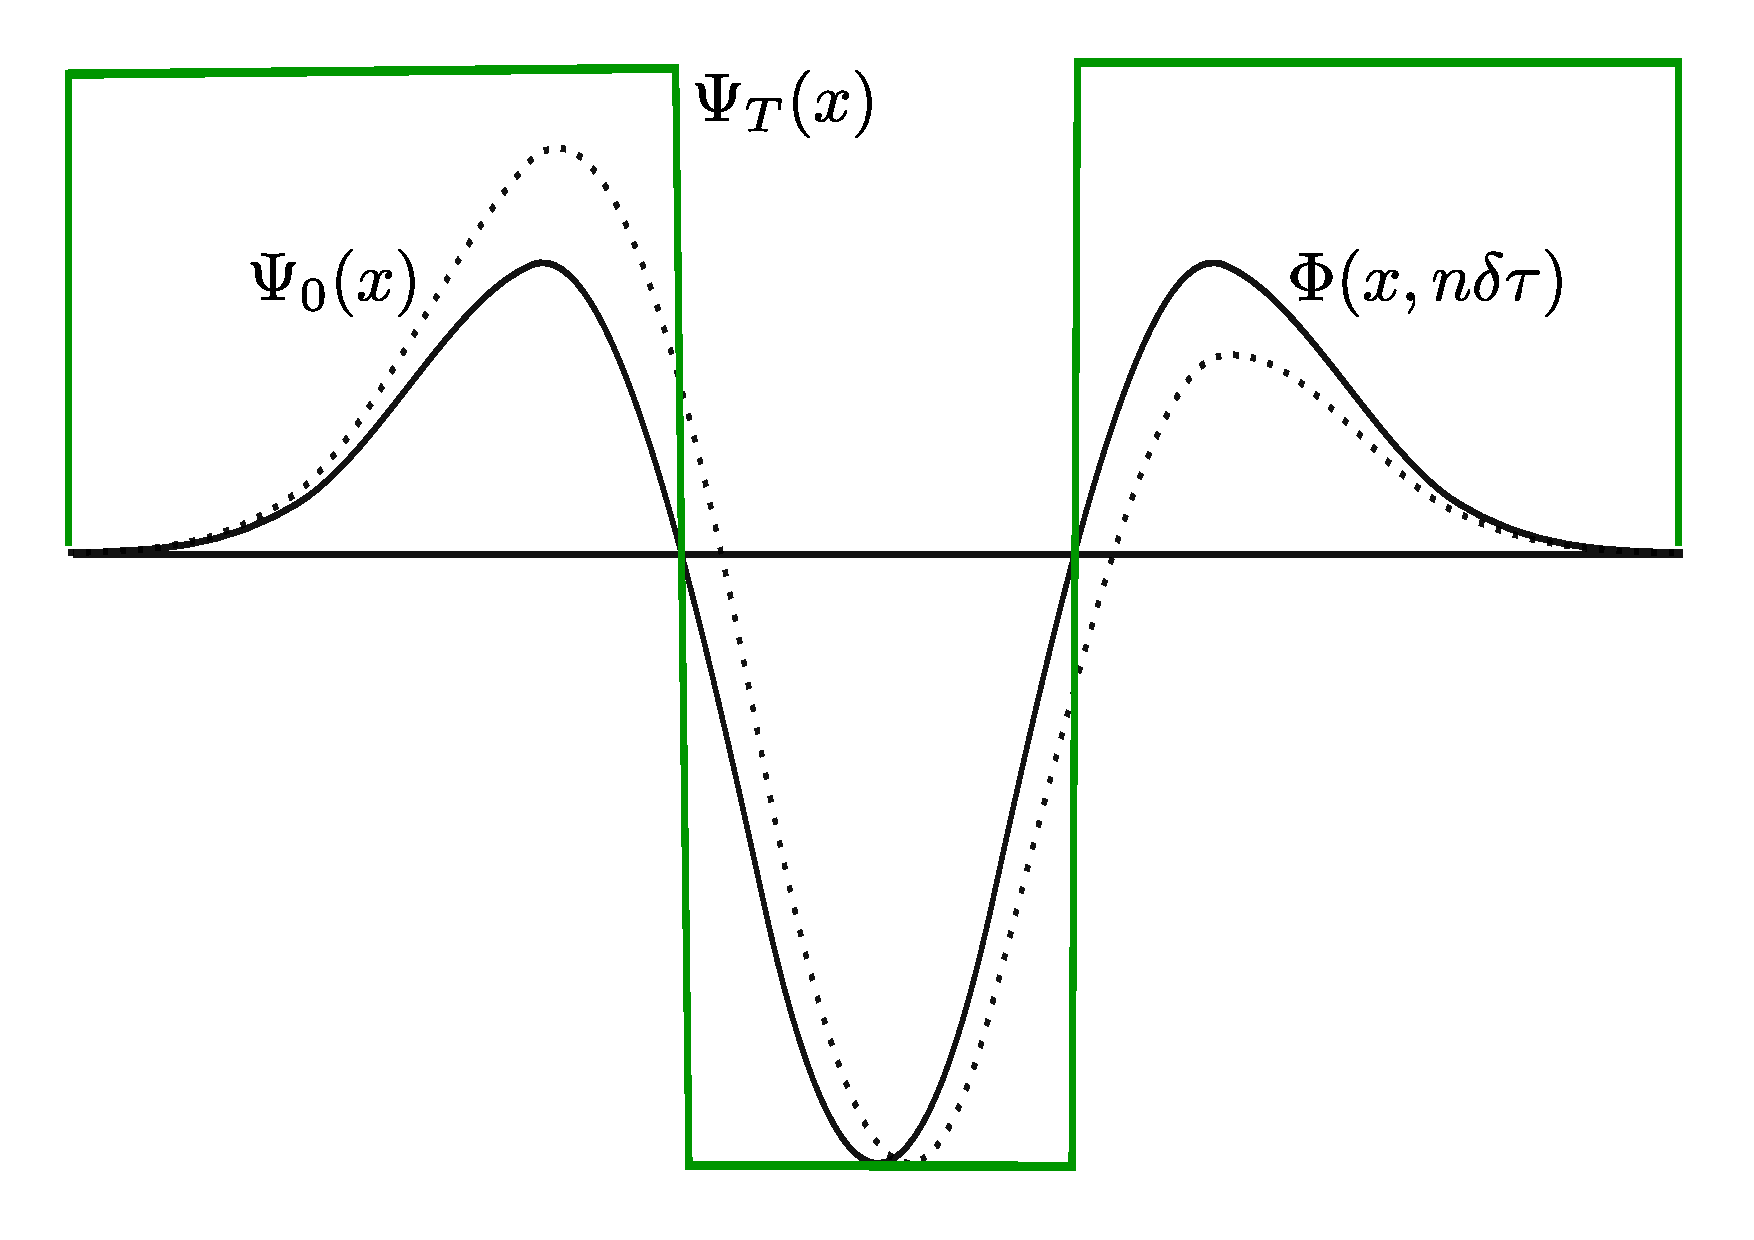
\includegraphics[scale=0.3]{../graphics/fixxednode.pdf}
 \end{center}
 \caption{The fixed node approximation illustrated. The nodes of $\Phi(x, n\delta\tau)$ is fixed to match those of $\Psi_T(x)$.}
\end{figure}
\end{frame}


\begin{frame}
\frametitle{Branching}

\textbf{Idea}: The weights are modelled by spawning and killing walkers with a rate equal to $G_\mathrm{B}$. 
\shift

\textbf{Problem}: $G_\mathrm{B}$ is not necessarily an integer.
\shift

\textbf{Solution}: Create $\mathrm{floor}(G_\mathrm{B})$ copies with a $G_\mathrm{B} - \mathrm{floor}(G_\mathrm{B})$ chance of creating an additional copy.
\shift

Or more compact: Create 

\begin{equation}
\overline{G}_\mathrm{B} = \mathrm{floor}(G_\mathrm{B} + a)
\end{equation}

copies, where $a \in [0,\,1)$ is a uniformly distributed random number. If the value is zero, the walker dies.

\end{frame}


\begin{frame}
\frametitle{Branching}

\begin{figure}
\begin{center}
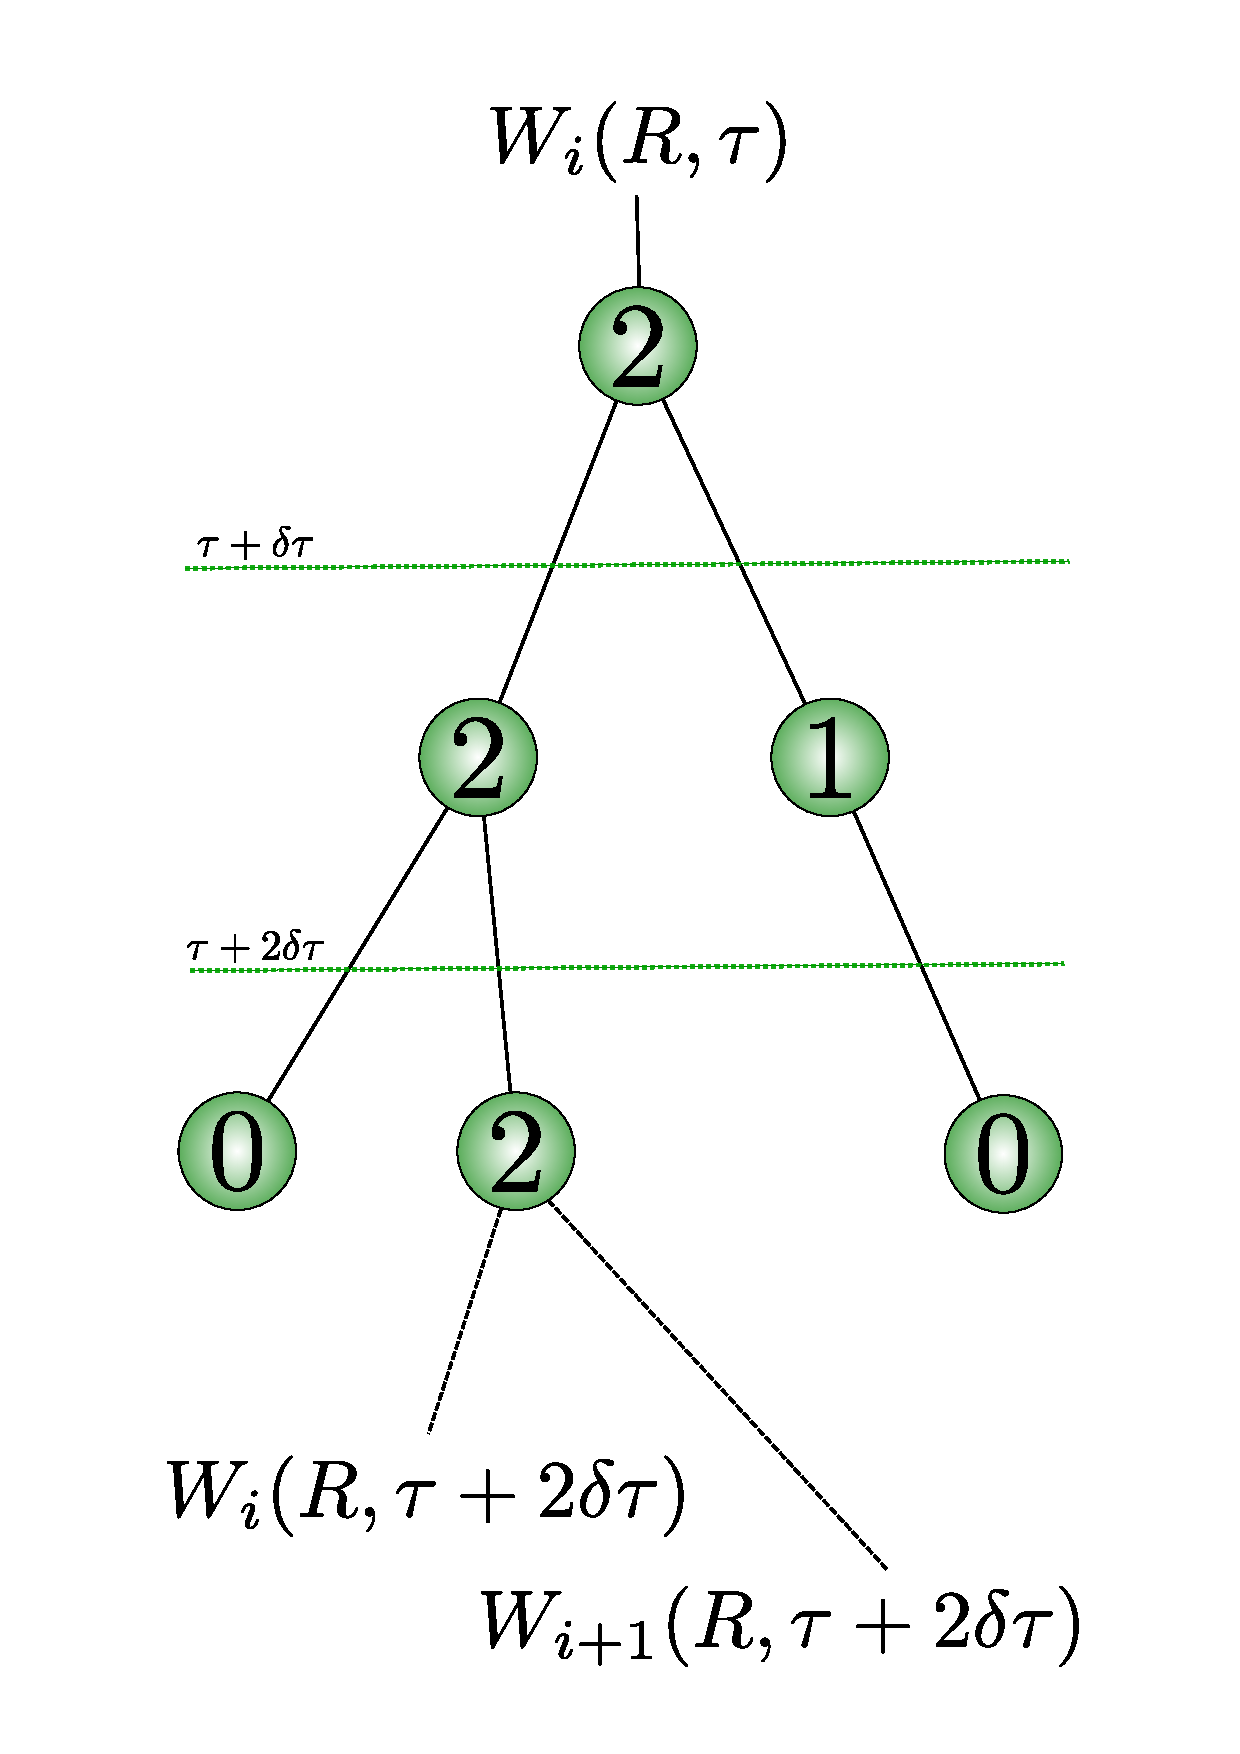
\includegraphics[scale=0.2]{../graphics/branching.pdf}
\end{center}
\caption{Branching illustrated. The integer values represent $\overline{G}_\mathrm{B}$.}
\end{figure}

\end{frame}

\begin{frame}
 \frametitle{Diffusion}
 
 The diffusion equation representing $G_\mathrm{Diff}$ is the so-called \textit{Fokker-Planck equation}. 
 \shift
 
 Anisotropic diffusion process. The quantum force pushes the walkers into regions of higher probability. 
 \shift
 
 According to the Fokker-Planck formalism, a new position $\mathbf{r}_{i+1}$ is calculated from the old one, $\mathbf{r}_i$, as follows
 
 \begin{equation}
  \mathbf{r}_{i+1} = \mathbf{r}_i + D\delta\tau\mathbf{F}(\mathbf{r}_i) + \mathbf{\xi}, 
 \end{equation}

where $\mathbf{\xi}$ is a vector of normal distributed random numbers with variance $\sqrt{2D\delta\tau}$.
 
\end{frame}

\begin{frame}
\frametitle{Diffusion}

\textbf{Problem}: Due to a finite time step, the previous equations do not guarantee convergence.  
\shift

\textbf{Solution}: The \textit{Metropolis algorithm} will correct this bias:  

\begin{equation}
  A(i\,\rightarrow\,j) = \min\{R_G(i\,\rightarrow\,j)R_\psi(i\,\rightarrow\,j)^2, \,1\},
\end{equation}

where $i\,\rightarrow\,j$ denotes a transition from state $i$ to state $j$, $A$ is the probability of accepting the transition, 

\begin{equation*}
 R_G(i\,\rightarrow\,j) = G_\mathrm{Diff}(\mathbf{r}_{j}, \mathbf{r}_{i}; \delta\tau)/G_\mathrm{Diff}(\mathbf{r}_{i}, \mathbf{r}_{j}; \delta\tau),
\end{equation*}

and

\begin{equation*}
 R_\psi(i\,\rightarrow\,j) = |\Psi_T(\mathbf{r}_j)/\Psi_T(\mathbf{r}_i)|.
\end{equation*}

\end{frame}


%% 15

\begin{frame}
 \frametitle{Recap}
 
 \begin{itemize}
 \item The projection process is approximated by the diffusion of an ensemble of walkers with distributed weights.
 \pause \item Diffusion by the Fokker-Planck equation ensures efficient sampling by the use of the quantum force.
 \pause \item The Metropolis algorithm corrects the bias introduced by a finite step length. Ensures that the walkers follow $|\Psi_T(\mathbf{r})|^2$.
 \pause \item After each diffusion step, the walker is either killed or cloned based on the value of the branching Green's function. This ensures that the distribution of walkers follows $f(\mathbf{r}, \tau)$ and not $|\Psi_T(\mathbf{r})|^2$.
 \end{itemize}

\end{frame}

\subsection{Explicit methods}

\begin{frame}
 \frametitle{Variational Monte-Carlo}
 Neglecting the branching term results in a method known as \textit{Variational Monte-Carlo} (VMC).
 \shift
 
 Corresponds to calculating $\bra{\Psi_T}\OP{H}\ket{\Psi_T}$ using a standard Monte-Carlo approach
 
 \begin{equation}
  \bra{\Psi_T}\OP{H}\ket{\Psi_T} = \int_\mathbf{r} |\Psi_T(\mathbf{r})|^2 E_L(\mathbf{r})\mathrm{d}\mathbf{r} \simeq \frac{1}{N}\sum_{i=1}^N \frac{1}{\Psi_T(\mathbf{r_i})}\OP{H}\Psi_T(\mathbf{r}_i) 
 \end{equation}
  \shift
 
 Notice that using any other distribution than $|\Psi_T(\mathbf{r})|^2$ to sample the points $\mathbf{r}_i$ results in undefined samples of the local energy.

 
\end{frame}

\begin{frame}
 \frametitle{\textbf{Variational} Monte-Carlo}
 
 Variational Monte-Carlo will always result in an energy which is greater or equal to the exact ground state energy
 
 \begin{align*}
  \bra{\Psi_T}\OP{H}\ket{\Psi_T} &= \sum_{ij} C_i^\ast C_j \underbrace{\bra{\Psi_i} \OP{H} \ket{\Psi_j}}_{E_i\delta_{ij}} \\
                                 &= \sum_i |C_i|^2 E_i \\
                                 &= \sum_i |C_i|^2 (E_0 + \Delta E_i) \\
                                 &= E_0 \underbrace{\sum_i |C_i|^2}_{1} + \underbrace{\sum_i |C_i|^2\Delta E_i}_{\ge 0} \\
                                 &\ge E_0.
 \end{align*}
\end{frame}

\begin{frame}
 The \textit{variational principle} introduced in the previous slide opens up the possibility to introduce \textit{variational parameters} in $\Psi_T(\mathbf{r})$ whose values are found by minimizing the VMC energy in the parameter space.
 \shift
 
 Already have $\beta$ from the Jastrow factor. 
 \shift
 
 The \textit{spatial} wave function is modelled as a single \textit{Slater determinant}, which can be split into two parts $|\mathbf{S(\mathbf{r})}^\uparrow|$ and $|\mathbf{S(\mathbf{r})}^\downarrow|$ corresponding to two spin levels due to the fact that the Hamiltonian is assumed to be \emph{spin independent}.
 \shift
 
 Introducing the variational parameter $\alpha$ into the spatial wave function yields
 
 
 \begin{equation}
  \Psi_T(\mathbf{r}; \alpha, \beta) = |\mathbf{S(\mathbf{r}; \alpha)}^\uparrow||\mathbf{S(\mathbf{r}; \alpha)}^\downarrow|J(\mathbf{r}; \beta)
 \end{equation}

 
 
\end{frame}

\begin{frame}
\frametitle{Diffusion Monte-Carlo}
Including both diffusion and branching results in a method known as \textit{Diffusion Monte-Carlo} (DMC).
\shift

The DMC energy corresponds to the following integral

\begin{equation}
 E_{\mathrm{DMC}} = \frac{\int_\mathbf{r} f(\mathbf{r}, \tau) \frac{1}{\Psi_T(\mathbf{r})}\OP{H} \Psi_T(\mathbf{r})\mathrm{d}\mathbf{r}}{\int_\mathbf{r} f(\mathbf{r}, \tau)\mathrm{d}\mathbf{r}}  = \frac{\bra{\Phi(\tau)} \OP{H} \ket{\Psi_T}}{\braket{\Phi(\tau)}{\Psi_T}},
\end{equation}

\pause
which upon convergence of the projection results in $\OP{H}\ket{\Phi(\tau)} = E_0\ket{\Phi(\tau)}$. The energy becomes

\begin{equation}
 E_{\mathrm{DMC}} = \frac{\bra{\Phi(\tau)}E_0\ket{\Psi_T}}{\braket{\Phi(\tau)}{\Psi_T}} = E_0.
\end{equation}

\end{frame}

\begin{frame}
 \frametitle{Limitations: VMC}
 
 VMC is extremely robust, however, extremely dependent on a good ansatz for $\Psi_T(\mathbf{r})$.
 
\end{frame}

\begin{frame}
 \frametitle{Limitations: VMC}
 
 \begin{figure}
  \begin{center}
   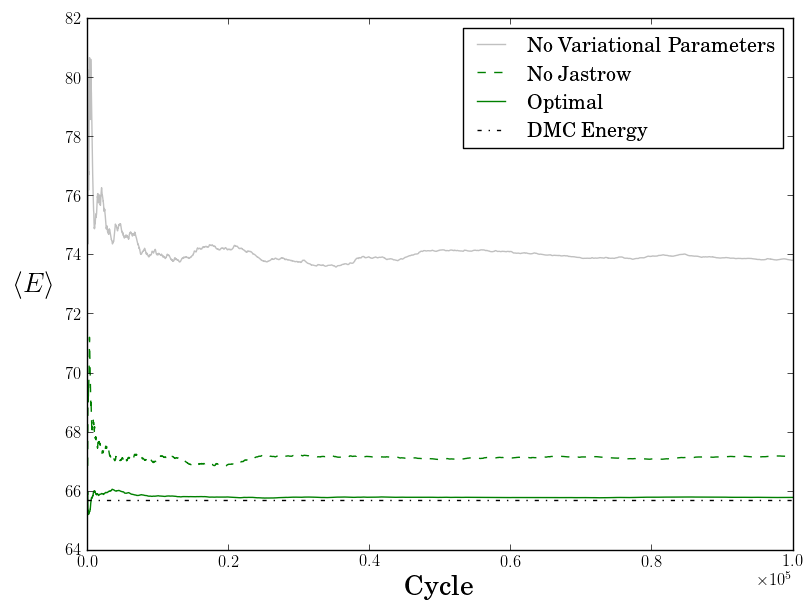
\includegraphics[scale=0.35]{../graphics/WFComp.png}
  \end{center}
  \caption{Comparison of different trial wave functions for a two-dimensional 12-particle quantum dot with unit frequency.}
 \end{figure}
 
\end{frame}


\begin{frame}
  \frametitle{Limitations: DMC}
  
  As discussed previously: The fixed node approximation.
  \shift
  
  \textbf{Problem}: The branching can get out of control for high \textit{variance} systems. 
  \shift
  
  \textbf{Solution}: Can be countered by choosing a lower time step. 
  \shift
  
  \textbf{Consequence}: Slower convergence. Breaking the requirement of \textit{ergodicity}.
  
\end{frame}

\begin{frame}
   \frametitle{Limitations: DMC}
   
   Diffusion Monte-Carlo is not as dependent on the trial wave function as VMC.
   
\end{frame}

\begin{frame}
 \begin{figure}
  \begin{center}
   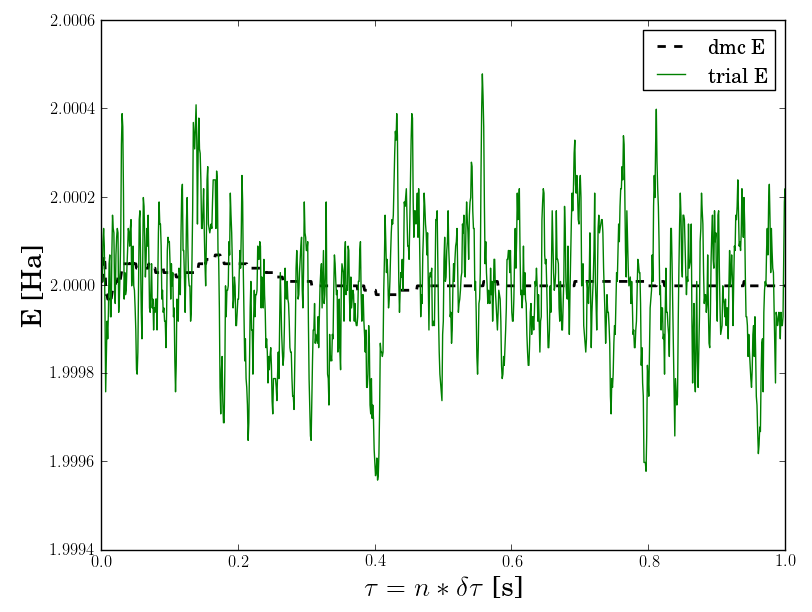
\includegraphics[scale=0.35]{../graphics/DMC_notExactWF.png}
  \end{center}
  \caption{DMC calculation without the exact wave function. The exact result is $E_0=2$. The VMC energy is $2.0042(3)$, whereas the DMC energy is $2.00000(2)$.}
 \end{figure}
\end{frame}

\subsection{Modelled systems}

\begin{frame}
 \frametitle{The modelled systems}
 \begin{itemize}
  \item Quantum dots
  \begin{itemize}
  \item Two dimensions
  \item Three dimensions
  \item Double wells
  \end{itemize}
  \pause
  \item Atomic systems
  \begin{itemize}
  \item Atoms
  \item Homonuclear Diatomic Molecules
  \end{itemize}
 \end{itemize}
\end{frame}

\begin{frame}
 \frametitle{Quantum dots}
 
 Quantum dots are interacting electrons in a harmonic oscillator potential
 
 \begin{equation}
  V_\mathrm{ext}(\mathbf{r}) = \frac{1}{2}\omega^2r^2,
 \end{equation}
 
 where $\omega$ is the oscillator frequency.
 
 \pause
 
 The harmonic oscillator eigenfunctions are
 
 \begin{equation}
  \phi_{n_x, n_y, n_z}(\mathbf{r}) = H_{n_x}(\sqrt{\omega}x)H_{n_y}(\sqrt{\omega}y)H_{n_z}(\sqrt{\omega}z)e^{-\frac{1}{2}\omega r^2},
 \end{equation}
 
 where $H_n(x)$ is the $n$'th level Hermite polynomial.


 
\end{frame}

\begin{frame}
 \frametitle{Quantum dots}
 
 Introducing a variational parameter $\alpha$ yields
 
 \begin{equation}
  \phi_{n_x, n_y, n_z}(\mathbf{r}; \alpha) = H_{n_x}(kx)H_{n_y}(ky)H_{n_z}(kz)e^{-\frac{1}{2}k^2r^2},
 \end{equation}
 
 where $k = \sqrt{\alpha\omega}$ represents the scaled oscillator potential.
 \shift

 \textbf{Problem}: With the electron-electron interaction these are no longer eigenfunctions of the Hamiltonian.
 \shift
 
 \textbf{Solution}: Quantum Monte-Carlo!
 
\end{frame}

\begin{frame}
 \begin{figure}
 \begin{center}
  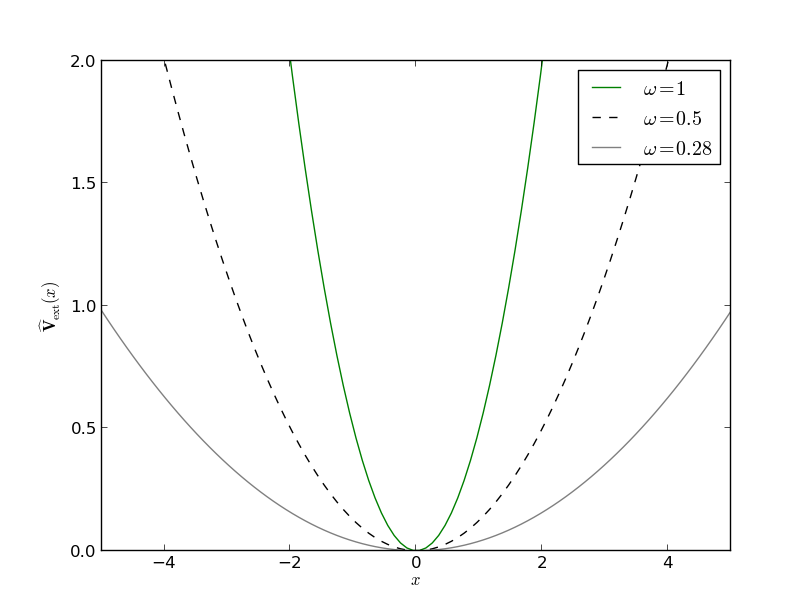
\includegraphics[scale=0.4]{../graphics/Potentials/qdots.png}
  \caption{A one-dimensional version of the single-particle potential of quantum dots.}
  \label{fig:extPotQDOTS}
 \end{center}
\end{figure}
\end{frame}

\begin{frame}
 \frametitle{Double wells}
 
 The double-well potential used is
 
 \begin{equation}
  V_\mathrm{ext}(\mathbf{r}) = \frac{1}{2}m^\ast \omega_0^2 \left[r^2 + \frac{1}{4}R^2 - R|x|\right], 
 \end{equation}

 where $R$ is the well separation, and $m^\ast$ and $\omega_0$ are material constants.
 \shift
 
 The construction of the new basis will be discussed later.
 
\end{frame}

\begin{frame}
 \begin{figure}
 \begin{center}
  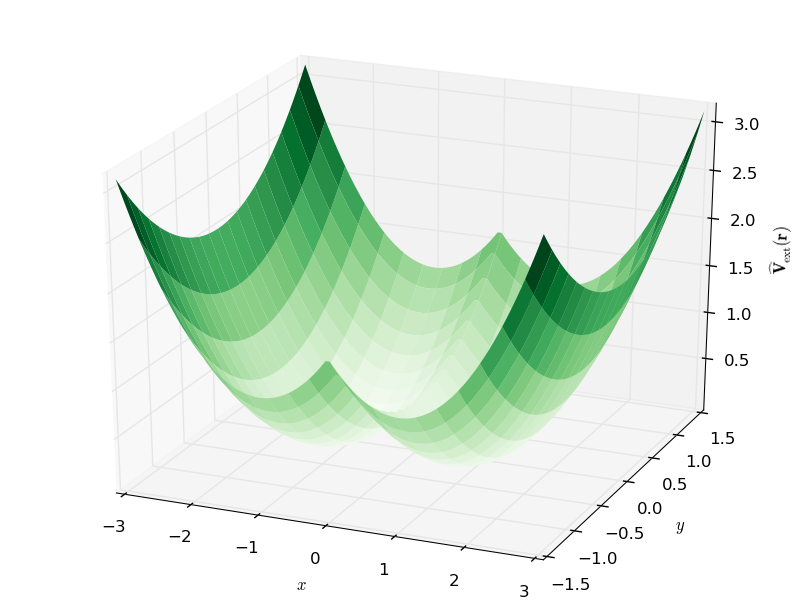
\includegraphics[scale=0.4]{../graphics/Potentials/doubleWell.png}
  \caption{The external potential for a double-well quantum dot.}
  \label{fig:extPotDoubleWell}
 \end{center}
\end{figure}
\end{frame}

\begin{frame}
 \frametitle{Atomic systems}
 
 Atomic systems are interacting electrons surrounding opposite charged nuclei. In the case of atoms, there is a single nucleus with charge $Z=N$. The potential used is
 
 \begin{equation}
 V_\mathrm{ext}(\mathbf{r}) = -\frac{Z}{r}. \label{eq:v0hydro}
\end{equation}
 \shift
 
 This corresponds to the hydrogen atom potential with the \textit{Born-Oppenheimer Approximation}.
 
\end{frame}

\begin{frame}
\begin{figure}
 \begin{center}
  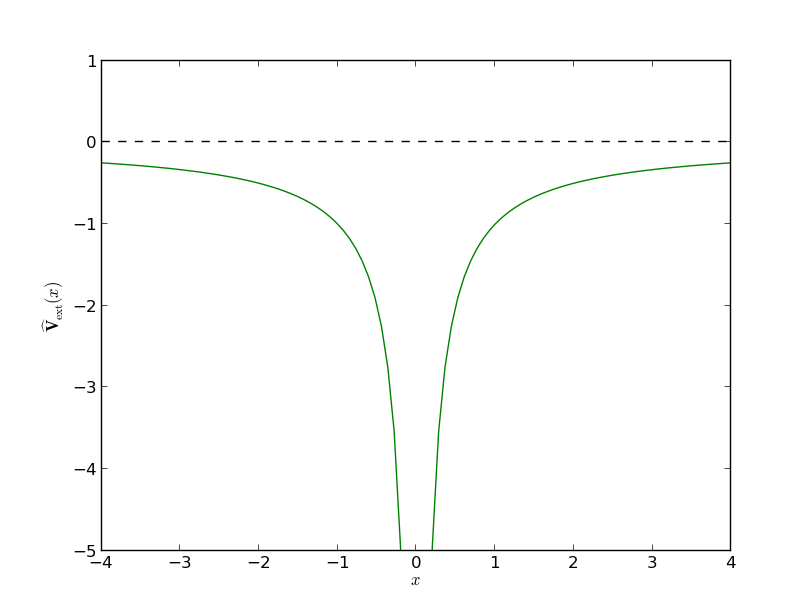
\includegraphics[scale=0.4]{../graphics/Potentials/hydrogen.png}
  \caption{The one-dimensional version of the single-particle potential of hydrogen.}
  \label{fig:extPotHydrogen}
 \end{center}
\end{figure}
\end{frame}

\begin{frame}
 The eigenfunctions are
 
 \begin{equation*}
 \phi_{nlm}(r, \theta, \phi; Z) \propto r^l e^{-Zr/n}\left[L_{n-l-1}^{2l+1}\left(\frac{2r}{n}Z\right)\right] Y_l^m(\theta, \phi), 
\end{equation*}

where $L_{q-p}^p(x)$ are the \textit{associated Laguerre polynomials} and $Y_l^m(\theta, \phi)$ are the \textit{spherical harmonics}. 
\shift
The spherical harmonics are related to the \textit{associated Legendre functions} $P_l^m$ in the following manner:

\begin{equation}
 Y_l^m(\theta, \phi) \propto   P_l^m(\cos\theta)e^{im\phi}. \label{eq:spherHarm}
\end{equation}

\end{frame}

\begin{frame}
 \textbf{Problem}: The spherical harmonics are complex functions. 
 \shift
 \textbf{Solution}: Use a special superposition of spherical harmonics known as the real-valued \textit{solid harmonics}
 
 \begin{align}
S_l^m(r, \theta, \phi) &\propto r^l\left[Y_l^m(\theta, \phi) + (-1)^m Y_l^{-m}(\theta, \phi)\right] \\
 &\propto r^{l} P_l^{|m|}(\cos\theta) \begin{cases} \cos m\phi & m \ge 0 \\ \sin|m|\phi &  m < 0 \end{cases}.     
\end{align}

 \end{frame}
 
 \begin{frame}
  The resulting eigenfunctions become 
  
\begin{equation*}
  \phi_{nlm}(r, \theta, \phi; k) \propto e^{-kr/n}\left[L_{n-l-1}^{2l+1}\left(\frac{2r}{n}k\right)\right] S_l^m(r, \theta, \phi) \equiv \phi^\mathrm{H}_{nlm}(\mathbf{r}), 
\end{equation*}

where $k = \alpha Z$ is a scaled charge with $\alpha$ as a variational parameter.
 \end{frame}

\begin{frame}
 \frametitle{Molecules}
 
 The Hamiltonian describing the homonuclear diatomic molecules is
 
 \begin{equation*}
 \OP{H}_{\mathrm{Mol.}}(\mathbf{r}, \mathbf{R}) = \sum_{i=1}^N \left[-\frac{1}{2}\nabla_i^2 + \frac{Z}{|\mathbf{r}_i + \mathbf{R}/2|} + \frac{Z}{|\mathbf{r}_i - \mathbf{R}/2|}\right] + \frac{Z^2}{R} + \sum_{i<j} \frac{1}{r_{ij}},
\end{equation*}

where $Z=N/2$ is the charge of the nuclei, $\mathbf{R}$ is the vector between the nuclei and $\mathbf{r}_i$ is the coordinates of electron $i$.
 
\end{frame}

\begin{frame}
 \begin{figure}
 \begin{center}
  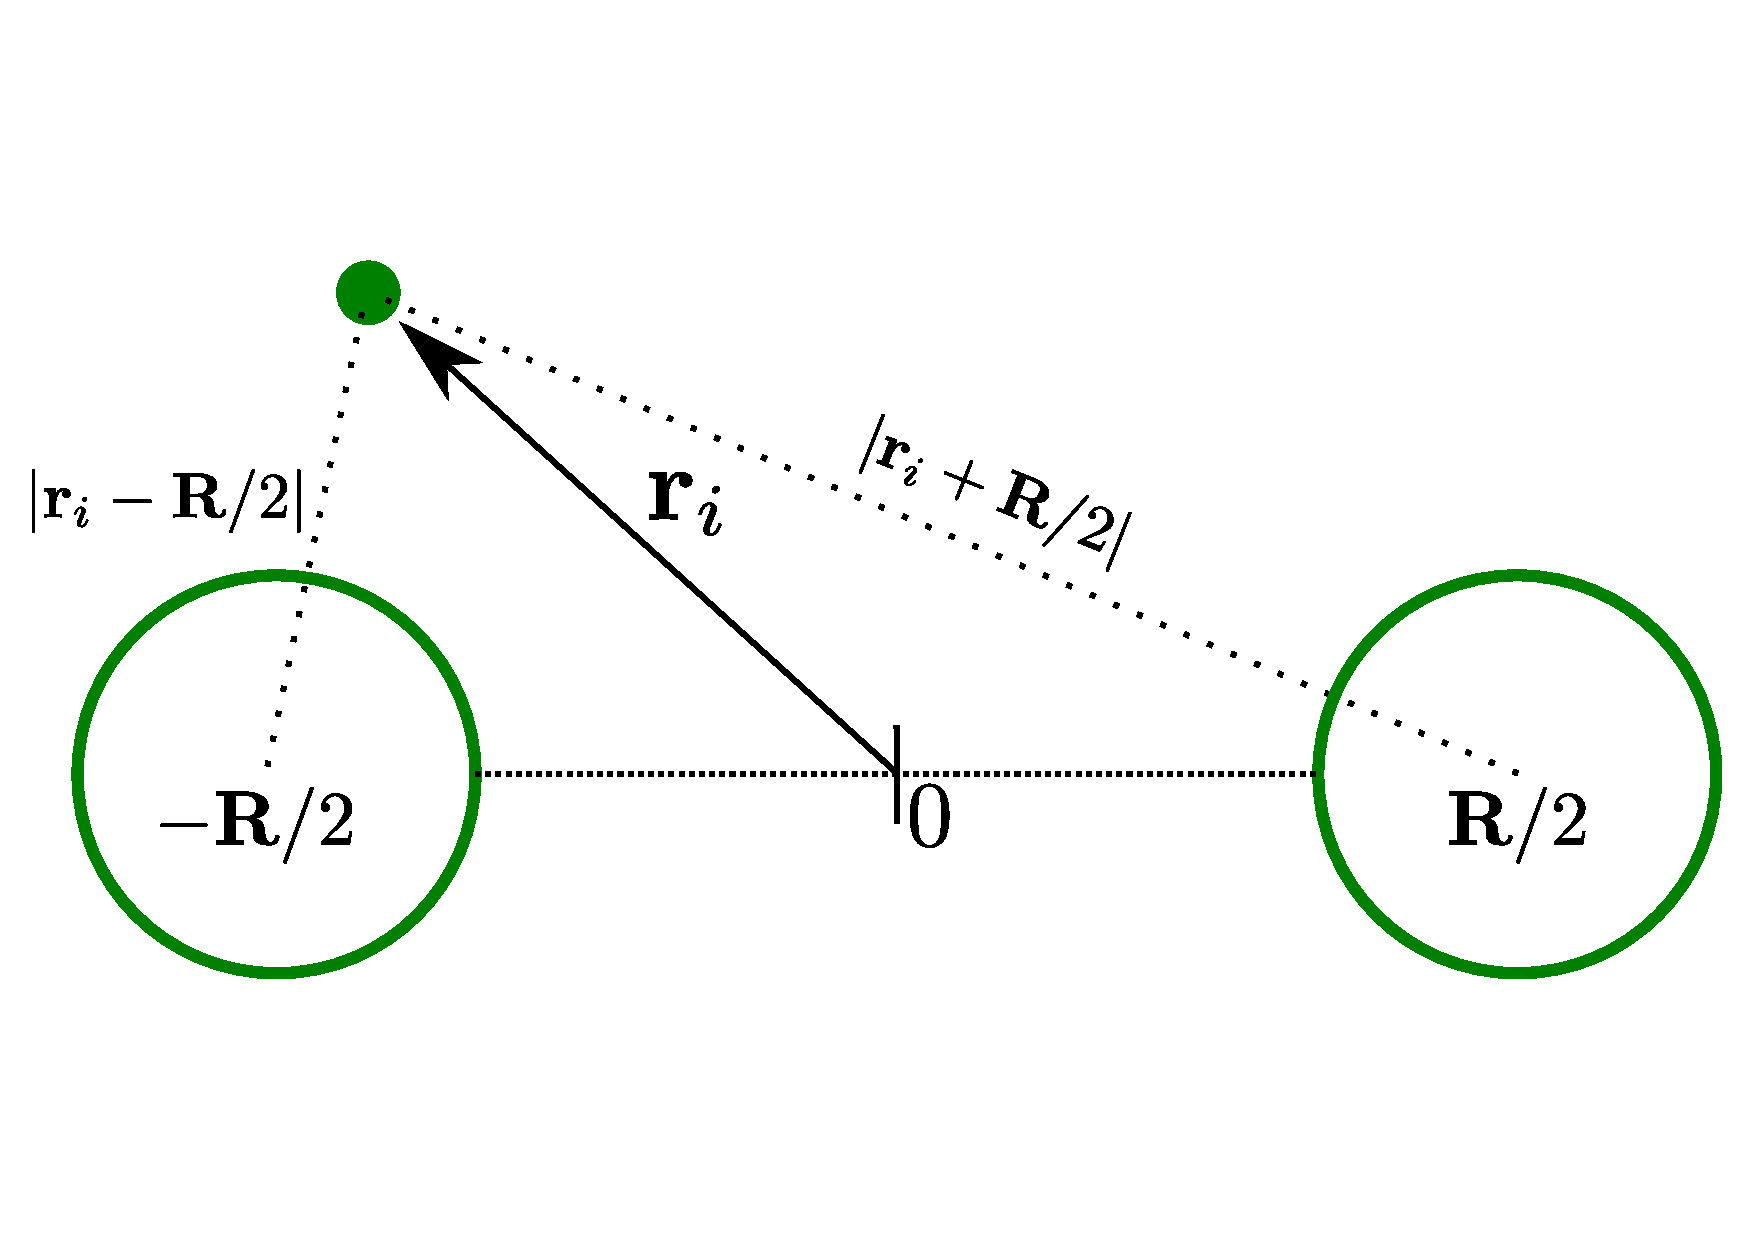
\includegraphics[scale=0.3]{../graphics/Molecules.pdf}
  \caption{The model for the diatomic molecule.}
 \end{center}
\end{figure}
\end{frame}

\begin{frame}
 In order to transform the hydrogen eigenstates $\phi_{nlm}^\mathrm{H}(\mathbf{r})$, which are symmetric around a single nucleus, into molecular single-particle states $\phi_{nlm}^\pm (\mathbf{r}_i)$, a superposition of the two mono-nucleus wave functions are used:

\begin{align*}
 \phi_{nlm}^+ (\mathbf{r}_i, \mathbf{R}) &= \phi_{nlm}^\mathrm{H}(\mathbf{r}_i + \mathbf{R}/2) + \phi_{nlm}^\mathrm{H}(\mathbf{r}_i - \mathbf{R}/2)\label{eq:moleculeTransPlus}, \\
 \phi_{nlm}^- (\mathbf{r}_i, \mathbf{R}) &= \phi_{nlm}^\mathrm{H}(\mathbf{r}_i + \mathbf{R}/2) - \phi_{nlm}^\mathrm{H}(\mathbf{r}_i - \mathbf{R}/2)\label{eq:moleculeTransMin}.
\end{align*}
\shift 

The same transformation are used to transform the harmonic oscillator eigenfunctions into the double well basis.

\end{frame}









